根据设计要求,本系统选用了目前最新的树莓派3B+作为主控模块,配合红外传感器、摄像头、步进电机及对应驱动芯片完成系统设计与开发。

\subsubsection{主控模块}
主控模块是系统的控制机构和通信机构,主要负责控制子模块的运行,处理信息及发送指令;与云服务系统进行通信,上传待识别车牌图像等原始信息,并接受云端指令。

本次停车场道闸控制系统选择了基于ARM嵌入式平台、树莓派系列中最新一代的树莓派3B+作为主控模块。树莓派3B+开发板拥有良好的标准模块扩展性,具备多种规格的外接设备口,主板上预留的接口可与树莓派500万像素专用摄像头完美对接,同时兼容红外传感器、步进电机等其他硬件开发模块。树莓派3B+实物如图\ref{fig:树莓派3B+实物图}所示。

\begin{figure}[htbp]
	\centering
	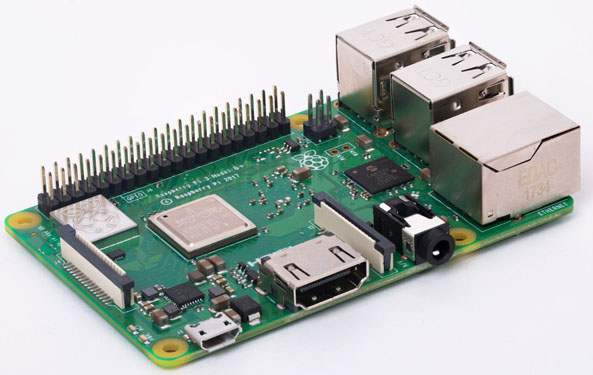
\includegraphics[width=\textwidth]{figure/hardware-RPI3B.jpg}
	\caption{树莓派3B+实物图}\label{fig:树莓派3B+实物图}
\end{figure}

树莓派3B+开发板是一款基于Broadcom BCM2837B0四核A53 CPU的多功能硬件开发平台,拥有1GB LPDDR2内存,采用Micro-SD作为外部存储,支持千兆以太网、2.4GHz和5GHz 双频Wi-Fi、蓝牙4.2,该开发板具有4个USB接口、一个以太网接口、HDMI高清视频输出接口、3.5mm模拟音频视频插孔、摄像机串行接口(CSI)、显示器串行接口(DSI)、40引脚GPIO双排插针,拥有强大的外接扩展能力和深度开发潜力。

树莓派将Python作为主要编程语言,支持java、BBC BASIC(通过RISCOS映像或者Linux的“Brandy Basic”克隆)、C和Perl等编程语言。本系统采用树莓派官方的最新Raspberry Pi系统(基于Linux32位操作系统开发而出),以Python作为编程语言完成系统开发。

\subsubsection{感应模块}
感应模块选用了红外传感器,其作用是检测车辆的到来,控制摄像头获取车牌图像,以及检测车辆是否通过道闸,道闸杆是否可以落下。红外传感器在待机状态时,持续输出为高电平;当红外传感器检测到物体时,会快速切换为工作模式,输出低电平;当物体被移开,红外传感器再次进入待机状态,输出高电平。红外传感器电路原理图如图\ref{fig:红外传感器原理图}所示。

\begin{figure}[htbp]
	\centering
	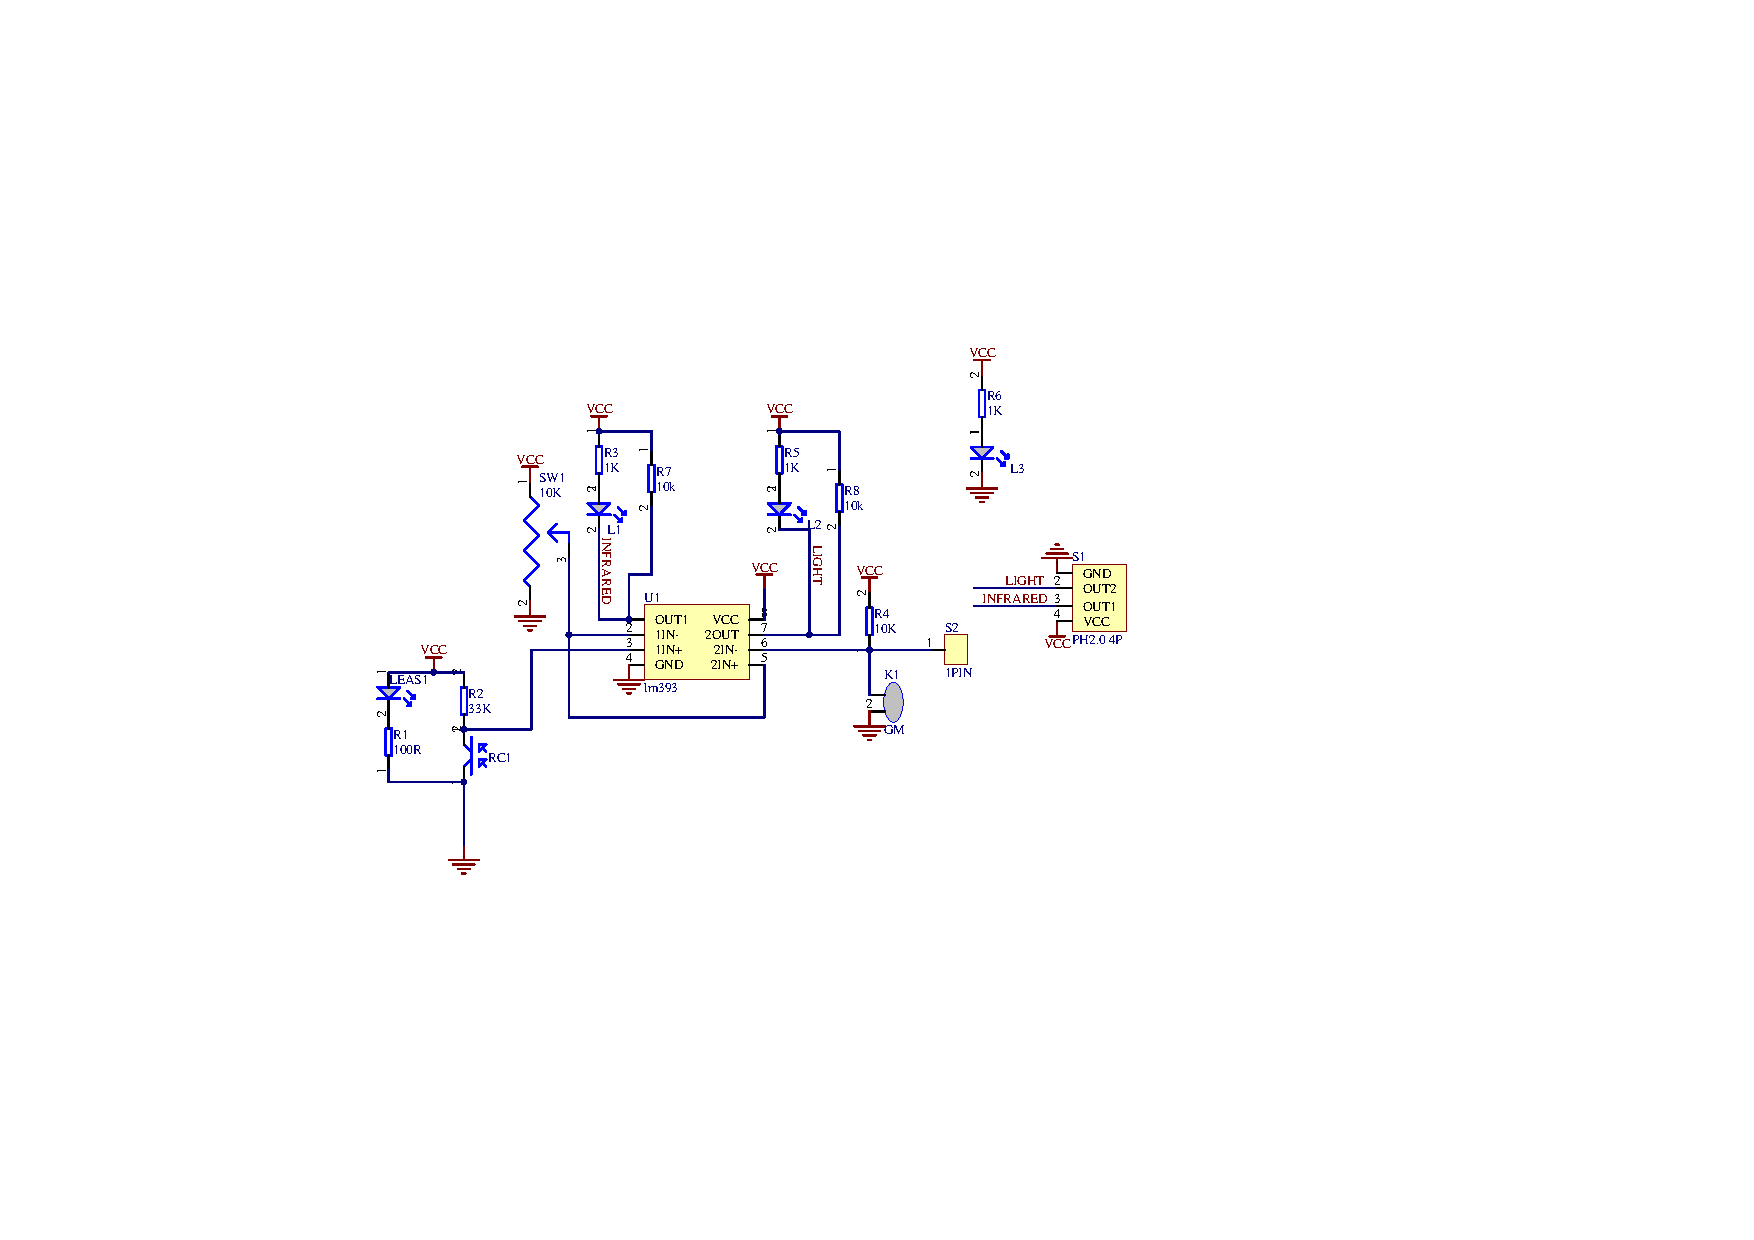
\includegraphics[width=\textwidth]{figure/hardware-red.pdf}
	\caption{红外传感器原理图}\label{fig:红外传感器原理图}
\end{figure}

\subsubsection{拍照模块}
拍照模块选用了树莓派专用500W像素摄像头(含CSI接口排线),该摄像头由OmniVision公司生产(基于OV5647图像处理传感模块),为树莓派专用拍照模块,兼容性更加优良。摄像头实物与参数如图\ref{fig:摄像头实物及参数图}所示。

\begin{figure}[htbp]
	\centering
	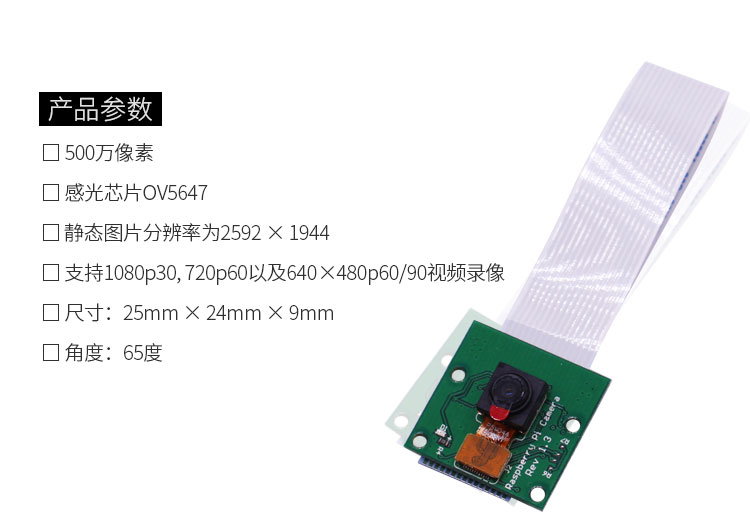
\includegraphics[width=\textwidth]{figure/hardware-camera.jpg}
	\caption{摄像头实物及参数图}\label{fig:摄像头实物及参数图}
\end{figure}

该拍照模块的核心元件是一个500W像素的CMOS传感器,支持最大分辨率为2592×1944的图片拍摄,同样支持每秒30帧的1080P视频拍摄(同时兼容每秒60帧的720P视频拍摄)。拍照模块与主控模块通过一条15芯的排线(CSI接口)进行连接。

\subsubsection{驱动模块}
由于树莓派的GPIO口驱动能力相对较弱,驱动电平仅为3.3V,所以高电平驱动比低电平驱动能力稍弱些。当主控模块直接将输入信号传递给步进电机时,步进电机无法正常工作,所以在本次设计中需要添加一个驱动模块。驱动模块具有放大功率的作用,可以满足在输入信号比较微弱、输出功率比较高的情况下工作。
考虑本系统实际,驱动模块主要需要满足以下要求:

\begin{itemize}
	\item 驱动电路提供的电流波形尽可能的接近矩形波,需要电流的快速上升及快速下降;
	\item 驱动电路输出的功率及运行的效率要求较高,使系统提高运行经济效率。
\end{itemize}

经过简单的比对,本系统设计拟采用ULN2003类的驱动IC(集成电路芯片),该芯片可为步进电机提供小于0.5A的电流。驱动芯片ULN2003内部结构如图\ref{fig:ULN2003内部控制单元原理图}所示。

\begin{figure}[htbp]
	\centering
	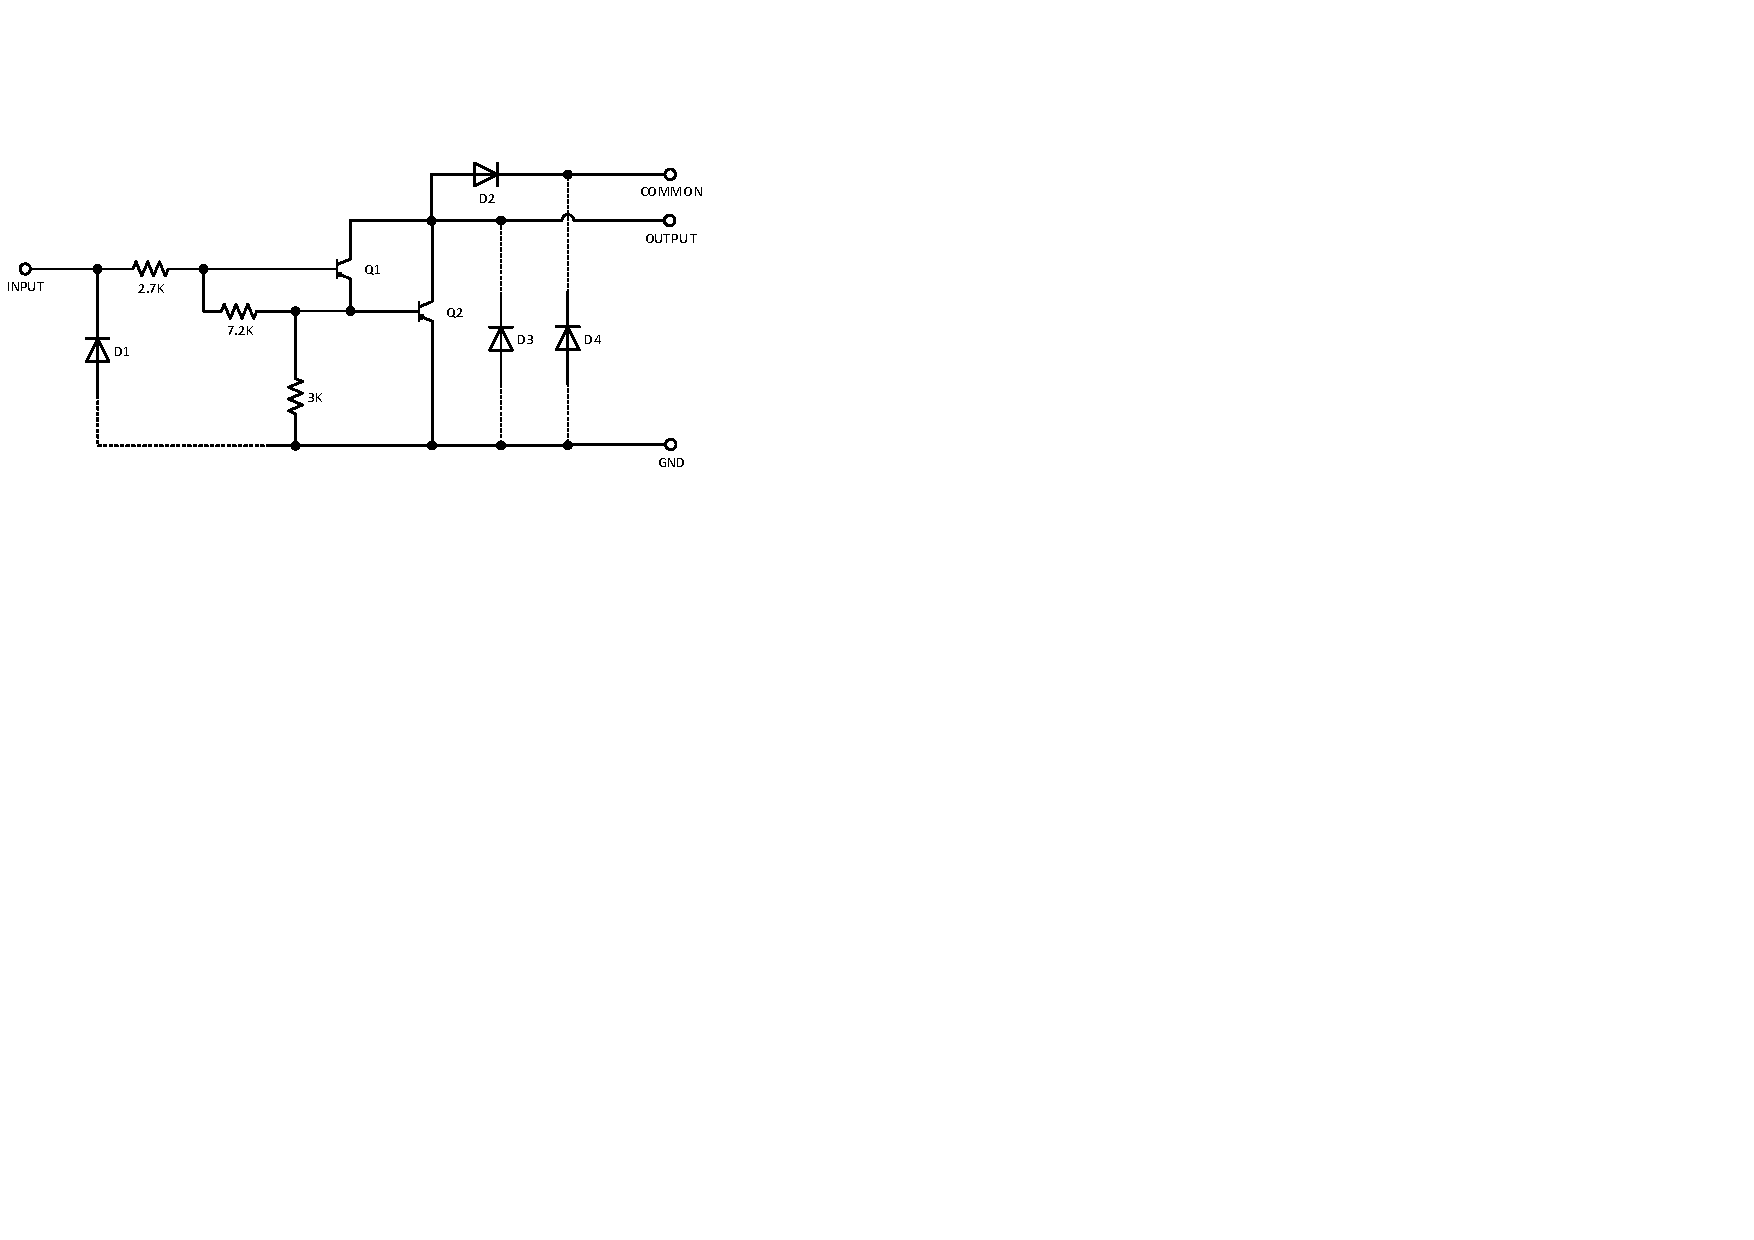
\includegraphics[width=\textwidth]{figure/hardware-cir.pdf}
	\caption{ULN2003内部控制单元原理图}\label{fig:ULN2003内部控制单元原理图}
\end{figure}

ULN2003芯片是由多个复合达林顿晶体管排列组成,这样的设计可以使耐受电压比较高,允许通过电流比较大。该芯片由7对NPN达林顿管组成,每个NPN达林顿管作为1个控制单元,其中7个控制单元包含功率驱动单元、保护单元等。ULN2003采用多种封装方式:如DIP-16或者SOP-16双列16脚塑料封装。驱动模块输出端可以与步进电动机直接连接,其内部数字逻辑电路为非门电路,采用取反的控制方式。

在满足以上要求的同时,系统还要稳定运行且性价比高,所以系统最终采用 ULN2003 作为电机驱动芯片。该芯片可以直接使用主控模块的GPIO口所提供的信号,硬件电路连接十分简单。该芯片采用树莓派作为控制核心,在进行程序相互调用时,操作起来也十分方便灵活。

ULN2003芯片的主要特点是:
\begin{itemize}
	\item ULN2003芯片驱动电流比较大,可以较好的用于单片机控制的电路。
	\item 为提高其抵抗干扰的能力,ULN2003可通过连接上拉电阻的方式,在驱动步进电机时抵御不必要的干扰。同时芯片内部每个控制单元都会串联高阻值的电阻,这样可以直接与TTL或承载电压为5V的CMOS装置连接。
	\item ULN2003输出端的电路集电极状态设置为开路状态,优点是电流的输出值比较大,峰值可以达到500mA,因此可以用来驱动步进电机。
\end{itemize}

ULN2003芯片引脚如图\ref{fig:ULN2003原理图}所示,输入部分为左侧1~7引脚,连接主控模块输出端(GPIO),由主控模块提供控制信号;引脚8直接接地;输出部分为右侧1~7引脚,与5V步进电机相连,必要时可以悬空而置,不做任何连接;引脚VCC接5V电源,该芯片可提供最高为0.5A的电流输出。

\begin{figure}[htbp]
	\centering
	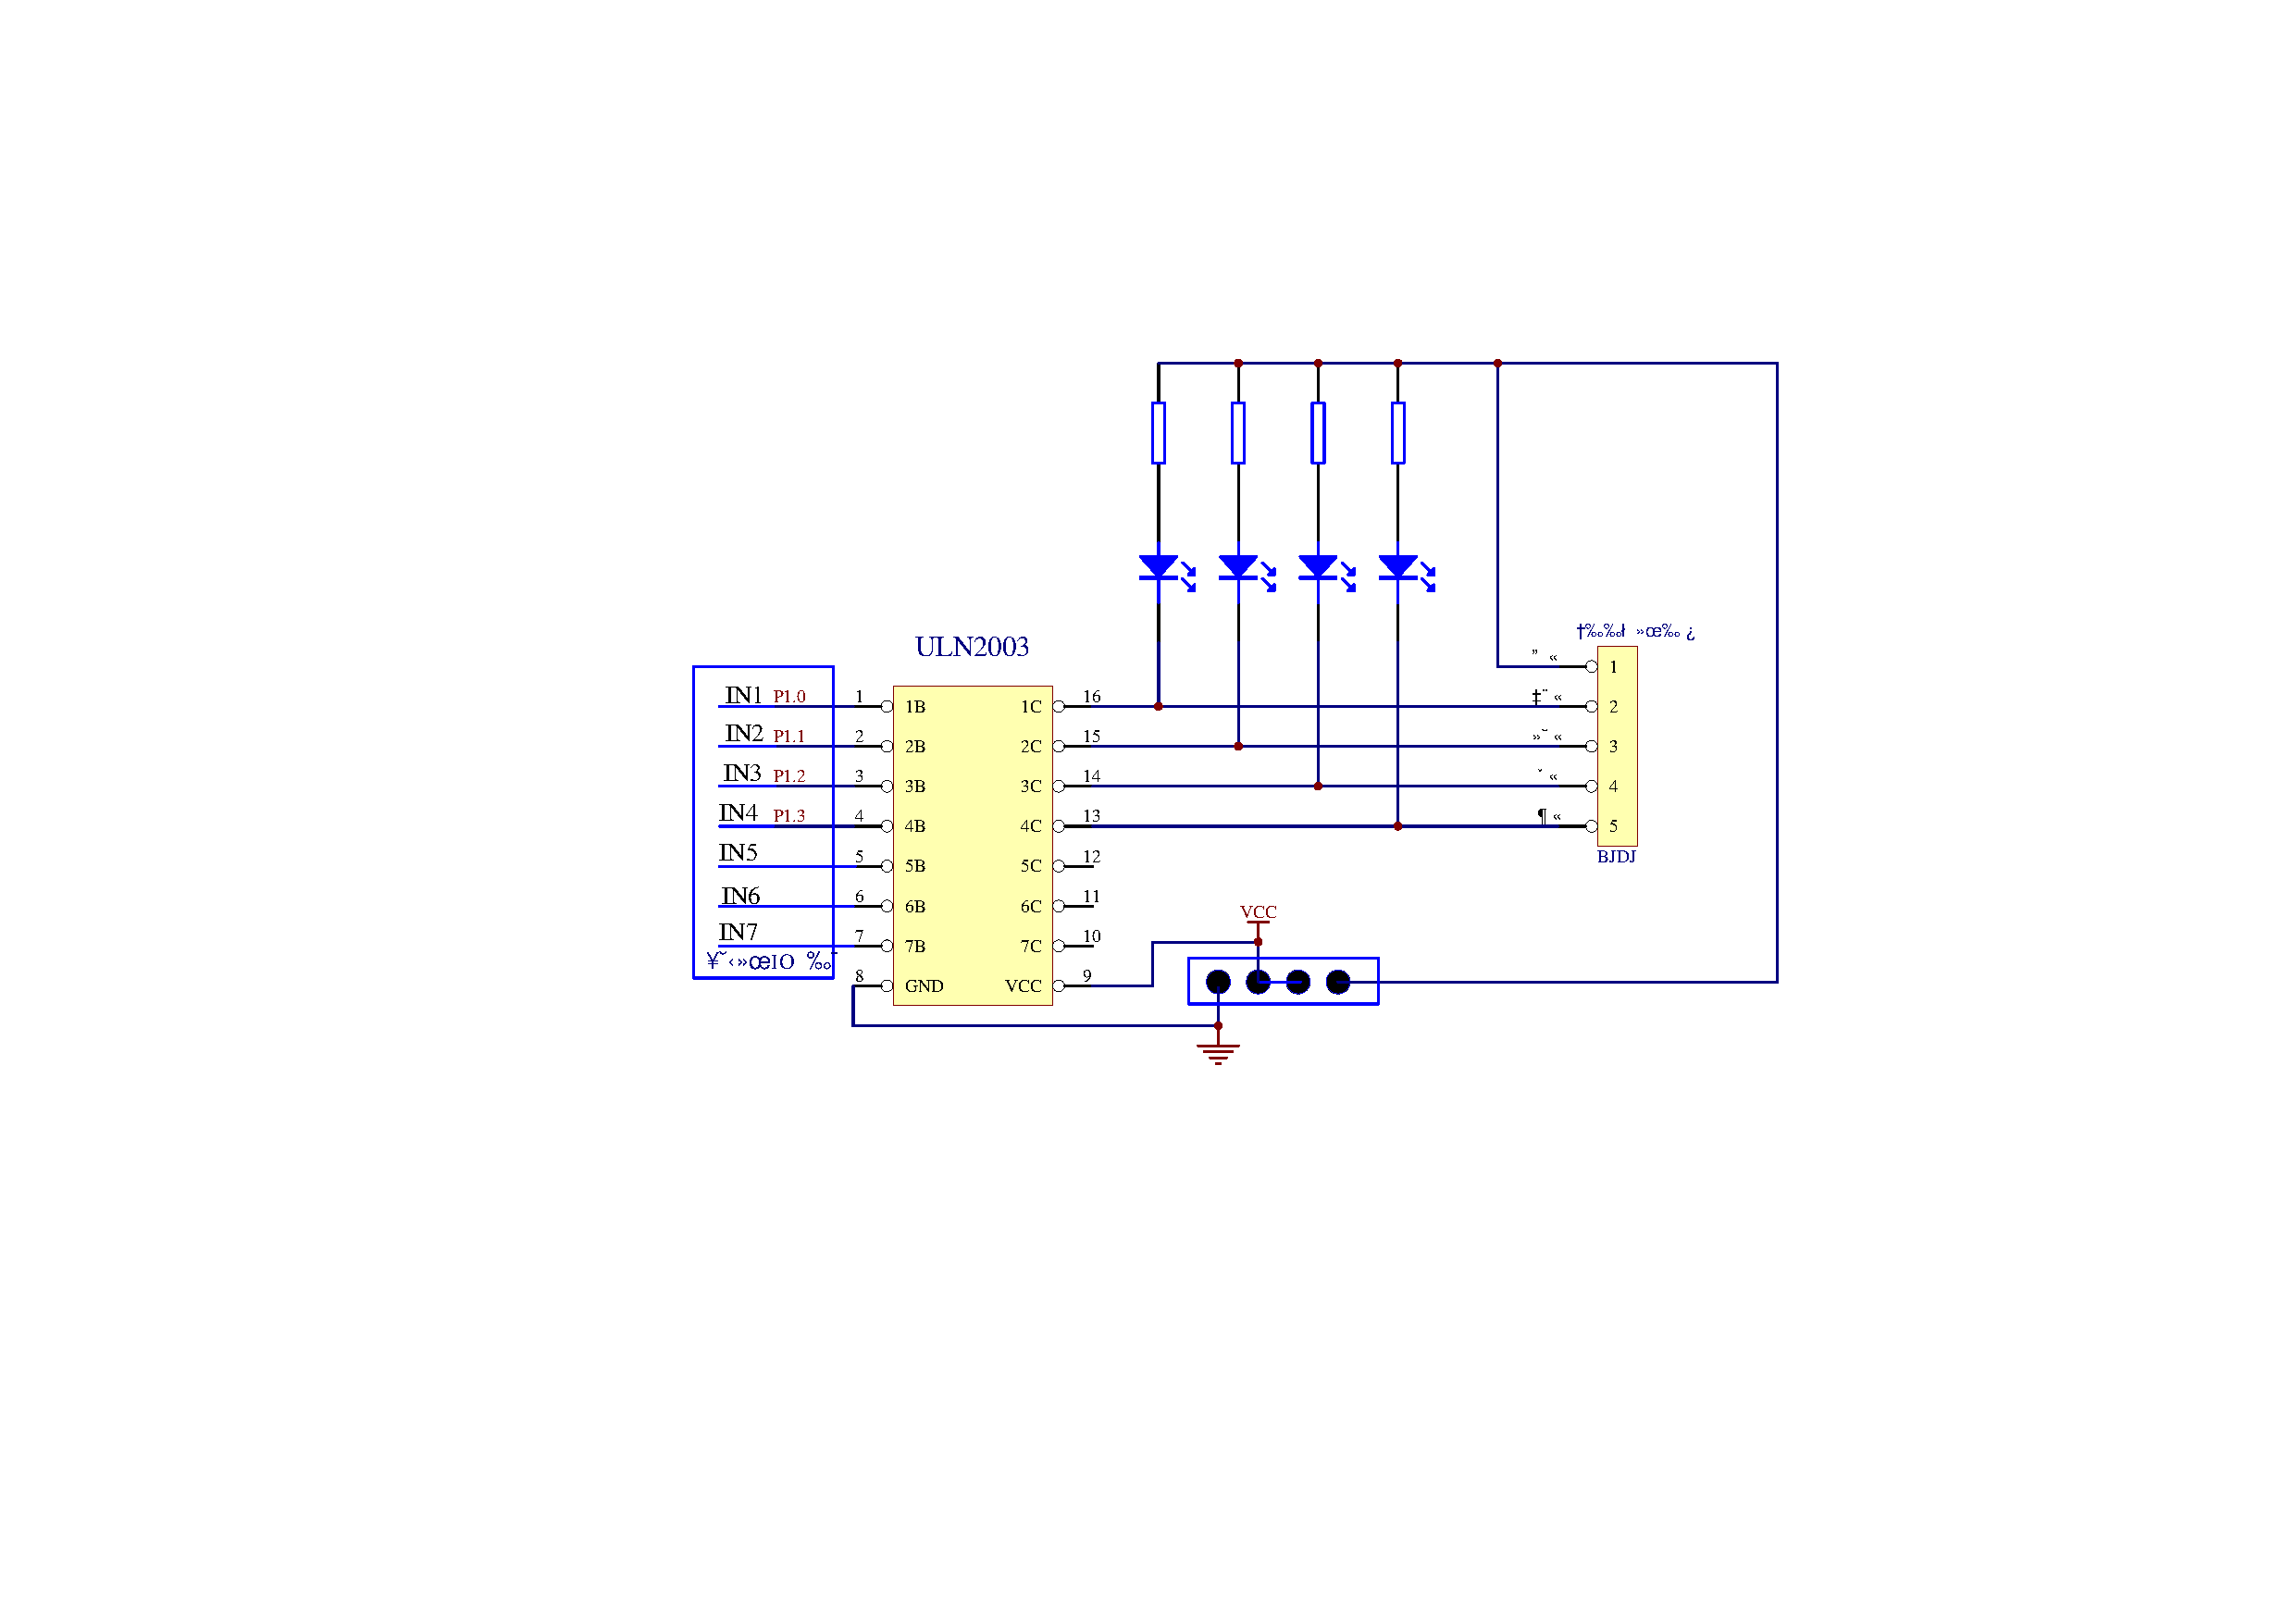
\includegraphics[width=\textwidth]{figure/hardware-pin.pdf}
	\caption{ULN2003原理图}\label{fig:ULN2003原理图}
\end{figure}

按照电路设计,步进电机输入端的红色线接VCC,其它线则用来连接驱动板。根据芯片资料,步进电机驱动芯片上有IN1~4四个接口,驱动方式为低电平供电,用杜邦线分别将 IN1,IN2,IN3,IN4 和GPIO 5(Pin 29),GPIO 6(Pin 31),GPIO 13(Pin 33),GPIO 19(Pin 35)进行连接。每次将四个GPIO端口按表2-3(步进电机驱动原理表)依次设置好电平后,可以通过设置sleep函数的时间来控制转速。

\subsubsection{电机模块}
步进电机属于电机中一个独特的类别,有别于常见的电机,该类别的电机具有精准控制的功能,可同时控制位置与速度两个矢量。与其他控制类电机不同的是,该种电机的控制方式采用开环控制(无反馈环节),可将输入端微弱且间断的触发脉冲信号转变成电机转动的线位移或者角位移。控制方式采用数字信号进行控制,短暂的脉冲信号就可对电机实现控制,随即转化为相应的角位移。由上得知,只要在步进电机输入端加以一个适当的脉冲信号,然后就会输出固定的角度,该种控制方式对开发者来说编程简单,操作可见性高。步进电机的相数取决于绕在定子的线圈数量,可分为两相、四相、五相等;步进电机的线式取决于电机的外部引线,分为三线式、五线式、六线式等。根据相数、线式、功能、用途的不同,步进电机分为多种类型,但是电机本身的控制方法均通过脉冲信号进行控制,没有很大的区分。

考虑到道闸系统的实际使用情况,运动过程中不需要加速、减速过程,同时对转速的要求也比较低,所以将步进电机设置为自启动运行方式。自启动运行方式是指通过控制脉冲速度,从而控制电机的启动和停止的运行方式,该种运行方式不会产生加速或者减速阶段。由于在道闸系统的开启、闭合时需要速度的突然变化,所以需要较大的转矩。同时在实际使用过程中电机有一定的负载,会产生较大的工作噪音,根据常见步进电机的工作特性,只有四相五线式步进电机的满足工作需求。另外考虑到静转矩、步距角、电流、安装难度等多种因素,本系统选取28BYJ-48四相五线式步进电机对道闸系统进行控制。